\hypertarget{ux4f7fux7528ux6a21ux677f}{%
\subsection{使用模板}\label{ux4f7fux7528ux6a21ux677f}}

Web 框架把我们从 WSGI 中拯救出来了。现在,我们只需要不断地编写函数,带上
URL,就可以继续 Web App 的开发了。

但是,Web App
不仅仅是处理逻辑,展示给用户的页面也非常重要。在函数中返回一个包含 HTML
的字符串,简单的页面还可以,但是,想想新浪首页的 6000 多行的
HTML,你确信能在 Python 的字符串中正确地写出来么?反正我是做不到。

俗话说得好,不懂前端的 Python 工程师不是好的产品经理。有 Web
开发经验的同学都明白,Web App 最复杂的部分就在 HTML 页面。HTML
不仅要正确,还要通过 CSS 美化,再加上复杂的 JavaScript
脚本来实现各种交互和动画效果。总之,生成 HTML 页面的难度很大。

由于在 Python 代码里拼字符串是不现实的,所以,模板技术出现了。

使用模板,我们需要预先准备一个 HTML 文档,这个 HTML 文档不是普通的
HTML,而是嵌入了一些变量和指令,然后,根据我们传入的数据,替换后,得到最终的
HTML,发送给用户:

 
 \begin{figure}[htp]
	\centering
	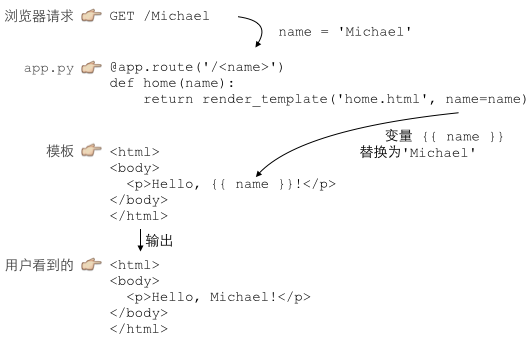
\includegraphics[width=0.6\linewidth]{fig/951383573211136.png}
\end{figure}


这就是传说中的 MVC:Model-View-Controller,中文名 ``模型 - 视图 -
控制器''。

Python 处理 URL 的函数就是 C:Controller,Controller
负责业务逻辑,比如检查用户名是否存在,取出用户信息等等;

包含变量\texttt{\{\{\ name\ \}\}}的模板就是 V:View,View
负责显示逻辑,通过简单地替换一些变量,View 最终输出的就是用户看到的
HTML。

MVC 中的 Model 在哪?Model 是用来传给 View 的,这样 View
在替换变量的时候,就可以从 Model 中取出相应的数据。

上面的例子中,Model 就是一个\texttt{dict}:

\begin{pythoncode}
{ 'name': 'Michael' }
\end{pythoncode}

只是因为 Python 支持关键字参数,很多 Web
框架允许传入关键字参数,然后,在框架内部组装出一个\texttt{dict}作为
Model。

现在,我们把上次直接输出字符串作为 HTML 的例子用高端大气上档次的 MVC
模式改写一下:

\begin{pythoncode}
from flask import Flask, request, render_template

app = Flask(__name__)

@app.route('/', methods=['GET', 'POST'])
def home():
    return render_template('home.html')

@app.route('/signin', methods=['GET'])
def signin_form():
    return render_template('form.html')

@app.route('/signin', methods=['POST'])
def signin():
    username = request.form['username']
    password = request.form['password']
    if username=='admin' and password=='password':
        return render_template('signin-ok.html', username=username)
    return render_template('form.html', message='Bad username or password', username=username)

if __name__ == '__main__':
    app.run()
\end{pythoncode}

Flask 通过\texttt{render\_template()}函数来实现模板的渲染。和 Web
框架类似,Python 的模板也有很多种。Flask 默认支持的模板是
\href{http://jinja.pocoo.org/}{jinja2},所以我们先直接安装 jinja2:

\begin{pythoncode}
$ pip install jinja2
\end{pythoncode}

然后,开始编写 jinja2 模板:

\hypertarget{home.html}{%
\subsubsection{home.html}\label{home.html}}

用来显示首页的模板:

\begin{pythoncode}
<html>
<head>
  <title>Home</title>
</head>
<body>
  <h1 style="font-style:italic">Home</h1>
</body>
</html>
\end{pythoncode}

\hypertarget{form.html}{%
\subsubsection{form.html}\label{form.html}}

用来显示登录表单的模板:

\begin{pythoncode}
<html>
<head>
  <title>Please Sign In</title>
</head>
<body>
  
  <p style="color:red">{{ message }}</p>
  
  <form action="/signin" method="post">
    <legend>Please sign in:</legend>
    <p><input {{ username }}"></p>
    <p><input ></p>
    <p><button type="submit">Sign In</button></p>
  </form>
</body>
</html>
\end{pythoncode}

\hypertarget{signin-ok.html}{%
\subsubsection{signin-ok.html}\label{signin-ok.html}}

登录成功的模板:

\begin{pythoncode}
<html>
<head>
  <title>Welcome, {{ username }}</title>
</head>
<body>
  <p>Welcome, {{ username }}!</p>
</body>
</html>
\end{pythoncode}

登录失败的模板呢?我们在\texttt{form.html}中加了一点条件判断,把\texttt{form.html}重用为登录失败的模板。

最后,一定要把模板放到正确的\texttt{templates}目录下,\texttt{templates}和\texttt{app.py}在同级目录下:

 
 \begin{figure}[htp]
	\centering
	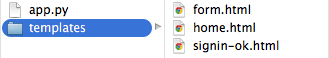
\includegraphics[width=0.6\linewidth]{fig/951386163120736.png}
\end{figure}


启动\texttt{python\ app.py},看看使用模板的页面效果:

 
 \begin{figure}[htp]
	\centering
	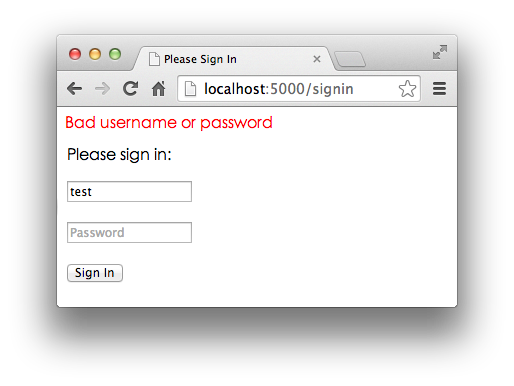
\includegraphics[width=0.6\linewidth]{fig/951385556253728.png}
\end{figure}


通过 MVC,我们在 Python 代码中处理 M:Model 和 C:Controller,而 V:View
是通过模板处理的,这样,我们就成功地把 Python 代码和 HTML
代码最大限度地分离了。

使用模板的另一大好处是,模板改起来很方便,而且,改完保存后,刷新浏览器就能看到最新的效果,这对于调试
HTML、CSS 和 JavaScript 的前端工程师来说实在是太重要了。

在 Jinja2
模板中,我们用\texttt{\{\{\ name\ \}\}}表示一个需要替换的变量。很多时候,还需要循环、条件判断等指令语句,在
Jinja2 中,用\texttt{\{\%\ ...\ \%\}}表示指令。

比如循环输出页码:

\begin{pythoncode}

    <a href="/page/{{ i }}">{{ i }}</a>

\end{pythoncode}

如果\texttt{page\_list}是一个
list:\texttt{{[}1,\ 2,\ 3,\ 4,\ 5{]}},上面的模板将输出 5 个超链接。

除了 Jinja2,常见的模板还有:

\begin{itemize}
\item
  \href{http://www.makotemplates.org/}{Mako}:用\texttt{\textless{}\%\ ...\ \%\textgreater{}}和\texttt{\$\{xxx\}}的一个模板;
\item
  \href{http://www.cheetahtemplate.org/}{Cheetah}:也是用\texttt{\textless{}\%\ ...\ \%\textgreater{}}和\texttt{\$\{xxx\}}的一个模板;
\item
  \href{https://www.djangoproject.com/}{Django}:Django
  是一站式框架,内置一个用\texttt{\{\%\ ...\ \%\}}和\texttt{\{\{\ xxx\ \}\}}的模板。
\end{itemize}

\hypertarget{ux5c0fux7ed3}{%
\subsubsection{小结}\label{ux5c0fux7ed3}}

有了 MVC,我们就分离了 Python 代码和 HTML 代码。HTML
代码全部放到模板里,写起来更有效率。

\hypertarget{ux6e90ux7801ux53c2ux8003}{%
\subsubsection{源码参考}\label{ux6e90ux7801ux53c2ux8003}}

\href{https://github.com/michaelliao/learn-python3/blob/master/samples/web/mvc/app.py}{app.py}

